\section{Integracja z jaskinią}
\sectionauthor{Stanisław Góra}
% LZWPLib
Przystosowanie aplikacji do działania w środowisku LZWP dzieli się na dwa podzadania: obsługa wejścia użytkownika oraz synchronizacja stanu aplikacji pomiędzy komputerami obsługującymi ściany jaskini. Reszta integracji jest zapewniana przez stworzoną przez pracowników LZWP bibliotekę.

% Input Module
\subsection{Moduł wejścia}
W założeniu aplikacja ma wspierać dwie metody interakcji użytkownika, nazywane później środowiskami:
\begin{enumerate}[label=\textbullet]
	\item \textbf{PC} - gdzie użytkownik posługuje się klawiaturą i myszą, używane głównie podczas procesu wytwarzania aplikacji
	\item \textbf{Jaskini} - gdzie użytkownik nosi okulary i trzyma specjalny kontroler nazywany flystickiem
\end{enumerate}
Aby ułatwić sobie wytwarzanie głównej logiki aplikacji, wejście zostało odseparowane w osobny moduł, który może być przed uruchomieniem ustawiony w jeden z dwóch trybów, odpowiadającym każdemu środowisku. Tryb ten definiuje jakiego rodzaju wejścia ma nasłuchiwać aplikacja. Moduł wejścia składa się z trzech mniejszych części:
\paragraph{Definicje akcji użytkownika}
Ustala wspólny interfejs dla każdej akcji użytkownika dostępnej w aplikacji. Są to między innymi: 
\begin{enumerate}[label=\textbullet]
	\item Użycie przycisku klawiatury i myszy (PC) lub flysticka (Jaskinia)
	\item Przesunięcie myszy (PC) lub flysticka (Jaskinia)
\end{enumerate}
Oprócz tego jest odpowiedzialna za nasłuchiwanie wykonania przez użytkownika swojej akcji i odpowiednie powiadomienie aplikacji.

\paragraph{Definicje akcji aplikacji}
Spis akcji wykonywanych w aplikacji. Są to między innymi: 
\begin{enumerate}[label=\textbullet]
	\item Wybranie lub podświetlenie węzła
	\item Poruszanie się po grafie
	\item Zmiana zakresu wyświetlanych połączeń
\end{enumerate}
Każda akcja ma swój typ (opisany w poprzednim punkcie). Dostępny jest też interfejs, dzięki któremu możliwe jest łatwe wybranie konkretnego przycisku (w każdym ze środowisk), który ma aktywować daną akcję (Rysunek \ref{fig:input-interface}).

\paragraph{Procesor akcji użytkownika}
Odpowiada za połączenie modułu wejścia z pozostałą częścią aplikacji poprzez powiadamianie jej o każdej wykonanej przez użytkownika akcji po ewentualnym wstępnym przetworzeniu sygnału wejściowego.


\img{\chapterPath/img/input-interface.png}{Fragment interfejsu wyboru przycisków dla środowiska PC}{input-interface}{.6}

% Networking
\subsection{Synchronizacja stanu}
Jak już zostało wspomniane, w LZWP każda ściana jaskini sterowana jest przez osobny komputer. Oznacza to, że środowisko aplikacji podobne jest do wieloosobowej gry w sieci LAN i wymusza synchronizację stanu z głównym komputerem, odpowiedzialnym za przetwarzanie akcji użytkownika. W tym celu powstał w aplikacji moduł wysyłający zmiany w grafie komputerom do aktualizacji ekranów. Cały proces zaprezentowany został na diagramie na Rysunku \ref{fig:diagram-modolow}.

Na opisanie zasługuje tu synchronizacja załadowanych lub usuniętych węzłów grafu. Mechanizm przesyłający wiadomości w sieci jest dosyć prosty i pozwala na dołączanie tylko najprostszych typów danych jak ciąg znaków, liczby i pozycja. Wysyłanie informacji o załadowaniu każdego węzła z osobna mogłoby zapełnić kanał komunikacyjny zwłaszcza przy starcie aplikacji, kiedy ładowane są tysiące węzłów na raz. Został więc wprowadzony mechanizm, którego celem jest zbieranie tych komunikatów i łączenie ich w większe paczki, które po przesłaniu są z powrotem rozpakowywane i przetwarzane. Dzięki temu aplikacja zachowuje optymalne wykorzystanie łącza w jaskini.

\begin{figure}[H]
\begin{center}
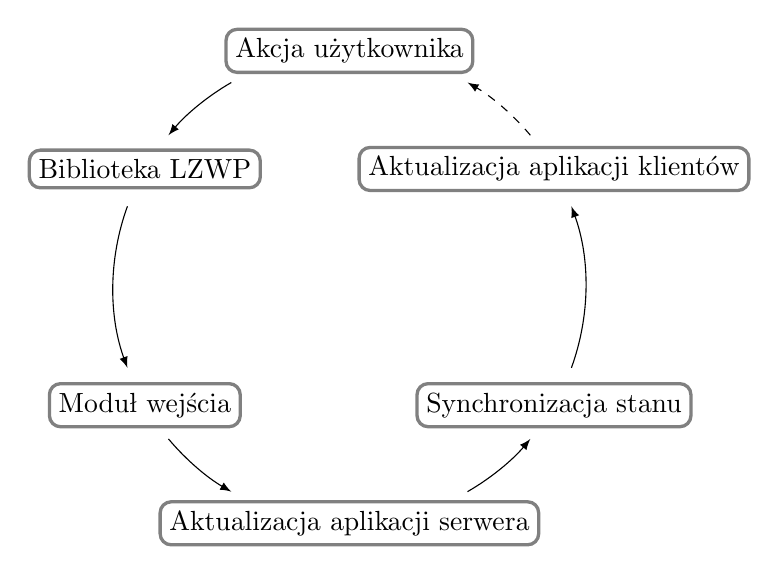
\begin{tikzpicture}[stepstyle/.style={rectangle, 
		rounded corners, draw=gray, very thick,
		text centered, align=center}]
	\def \n {6}
	\def \offset {30}
	\def \radius {3cm}

	\foreach \step [count=\s] in {Akcja użytkownika, Biblioteka LZWP, Moduł wejścia, Aktualizacja aplikacji serwera, Synchronizacja stanu, Aktualizacja aplikacji klientów} {
		\node(\s) [stepstyle] at ({360/\n * (\s) + \offset}:\radius) {\step};
	};
	\foreach \b/\e in {120/140, 160/200, 220/240, 300/320, 340/380} {
		\draw[->, >=latex] ({\b}:\radius)
		arc ({\b}:{\e}:\radius);
	};
		\draw[dashed, ->, >=latex] ({40}:\radius)
		arc ({40}:{60}:\radius);
\end{tikzpicture}
\end{center}
\caption{Diagram kolejności wykonywania modułów przy akcji użytkownika}
\label{fig:diagram-modolow}
\end{figure}


